\subsection{Possible Architectures and Related Diagrams}

\subsubsection{Proposed Sensor FOV Topology}
\noindent A ranging apparatus comprised of four ultrasonic sensors, one central LiDAR sensor, and optionally, a camera with spatial AI, should provide ample ability to FORWARD's object detection feature. Two wide FOV ultrasonic sensors face forward: one on each walker leg. Two face sideways, also mounted on the bottom half of the legs. The LiDAR sensor is mounted centrally so its beam detects straight-on obstacles. The camera is also mounted centrally. Finally, we angle these downward to allow for detection of obstacles present at the knee down height level. Additionally, a zero energy return from the ultrasonics or LiDAR could constitute a drop-off or ledge or divot. This will be elaborated upon in obstacle classification and identification.\\

\begin{figure}[H]
	\centering
	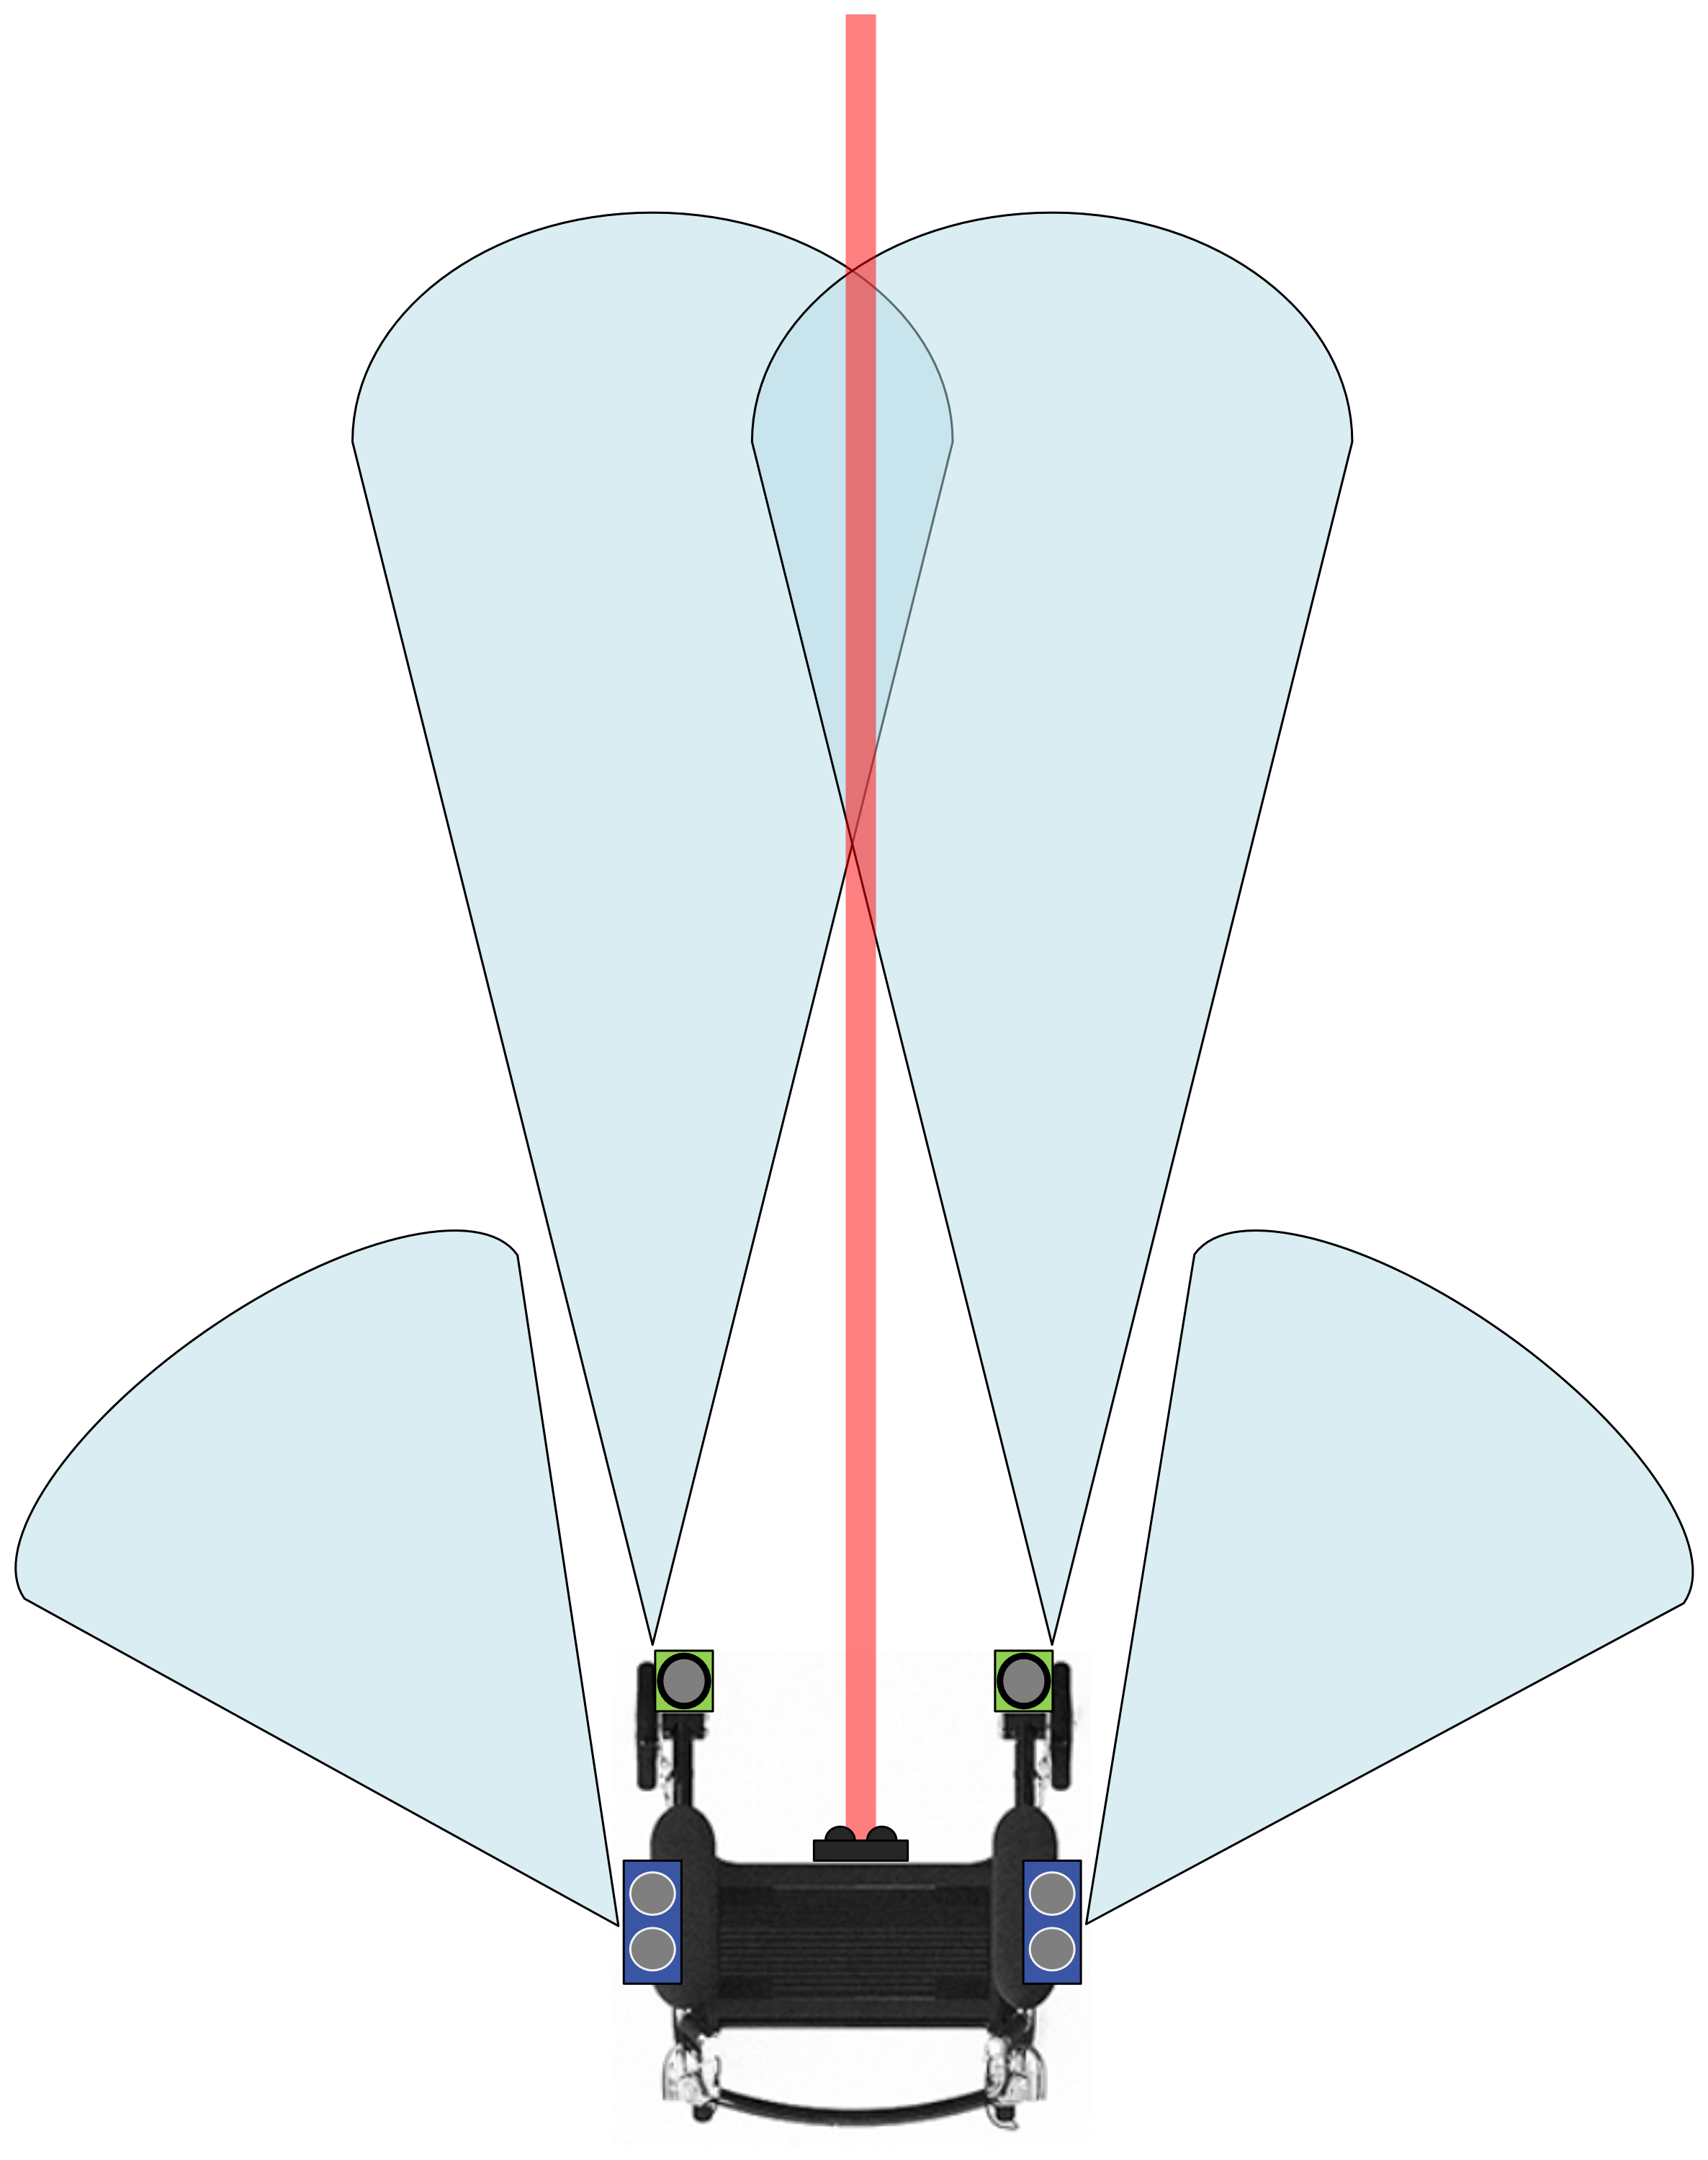
\includegraphics[angle=90,width=0.75\textwidth]{./Images/propose-sensorFOV.png}
	\caption{\label{fig:proposedsensorFOV}Proposed Sensor FOV (Range NOT to scale)}
\end{figure}

\noindent As mentioned in 2.2, the object detection data must work hand-in-hand with the identification and avoidance schemes. With identification, the range data is combined with any potential depth perception data generated by the camera. The closer the walker gets to the obstacle, the more urgently the system can respond. With avoidance, motor commands should be generated proportionately to the severity of the obstacle range-to-walker frame. Determining these specific plans of action is elaborated in later sections.\\

%\begin{figure}[h]
%	\centering
%	\includegraphics[width=0.7\textwidth]{./Images/FOVapparatus.png}
%	\caption{\label{fig:proposedFOVapparatus}Proposed Sensor Ranging Apparatus}
%\end{figure}

\subsubsection{Euler Angles}
\noindent Euler angles are one of our data streams that will inform FORWARD's guidance commands. We define a body reference frame whose center is the center of gravity of the rollator (with chassis and power supply mounted already). From there, we can monitor the \textit{attitude} $[\psi, \theta, \phi]$, or orientation, of the body frame, as represented by angles measured from the three major axes. The positive x-axis is defined as orthogonal to the front face of the rollator - in other words, forward looking-aft. Then, a positive rotation around this axis is defined as clockwise, or to the right, and results in a positive roll Euler angle, $\psi$. Next, we define the positive y-axis as perpendicular to the x-axis, using the right hand rule convention. A rotation about this axis is defined as positively clockwise, resulting in a positive pitch Euler angle, $\theta$. Finally, the positive z-axis is orthogonal to the xy-plane, and a positive rotation is rightwards. This results in a positive yaw Euler angle measurement $\phi$. We could theoretically define new reference frames, and perform coordinate transformations into those frames in order to gain new insight into the rollator attitude, but that is not necessary for the scope of this senior design project. We will simply monitor these angles to ensure stability, and aid the guidance of the user.\\

\subsubsection{Velocity and Position Solution}
\noindent With the addition of the IMU as indicated in section 3.3, FORWARD is able to resolve its relative velocity and position based on a starting point by twice integrating the accelerometer data output. By tracking these updates, FORWARD can be more self-aware of its current traveling state. Not only is the IMU useful for tilt detection (identifying incline and decline), but it can also be used to verify and validate the range data output by the LiDAR and sonar sensors. For example, the software can have some condition where, if the range decreases under a predetermined threshold of danger, then the IMU data can reset and begin tracking position and velocity, with that initial point as the origin of the reference frame. This can allow for very precise geometric abstracted data visualization of the free space ahead and the trajectory of the walker.\\

\subsubsection{Kalman Filter}
\noindent As part of the project stretch requirement for depth perception using an upgraded camera, implementation of a typical sensor fusion algorithm will help to predict the walker's trajectory and provide counteractive insight to the guidance system. Implementation of a Kalman filter estimator would not be beneficial for the fusion of the LiDAR and Sonar data, because the delta between these should be small, and thus, would not provide any helpful insight to FORWARD. However, if obtaining a second range solution from AI depth perception, this data could be fused to choose how much credence is given to either the standard range solution or the computer vision. Essentially, this functionality would be able to minimize measurement noise originating from the information loss of the sensors, and to maximize the overall precision of obstacle avoidance. \cite{kalman} \\

\noindent A Kalman Filter generates an estimation based on two measurements (that are likely noisy or deemed untrustworthy) by the following iterative algorithm:
\begin{enumerate}
	\item Initialize the state estimate and error covariance.
	\item Predict the next state and covariance based on previous states, covariance between successive measurements, and process noise (amount of credence given to either measurement).
	\item Update the measurement based on the Kalman gain.
\end{enumerate}

\subsubsection{Quaternions}
\noindent The BNO055 inertial measurement unit has a distinct advantage that involves a particularly interesting mathematical formulation. It is able to output quaternion data. Quaternions are a complex mathematical formulation which can be used as a replacement of sorts to \textit{Euler Angles}, mainly addressing the gimbal lock issue of Euler Angles, which occurs when two torus of rotation align and thus reduce the degrees-of-freedom. Quaternions generally are able to all for a smoother representation of rotations, using four dimensions (three imaginary) to transcend the three. \cite{quat} FORWARD will likely not make use of these, but they are quintessential in the field of guidance, navigation, and control, and thus warrant a mention in this study. See the fundamental representation:\\
$$i^2+j^2+k^2=ijk=-1$$

\noindent The quaternions could be useful for providing more precise navigation solutions than the angles as they can house more detailed information about the rollator's orientation. Most notably, on the data curves, they negate the 360 degree crossing. However, for the scope of meeting basic goals, it will not likely be needed.

\begin{figure}[H]
	\centering
	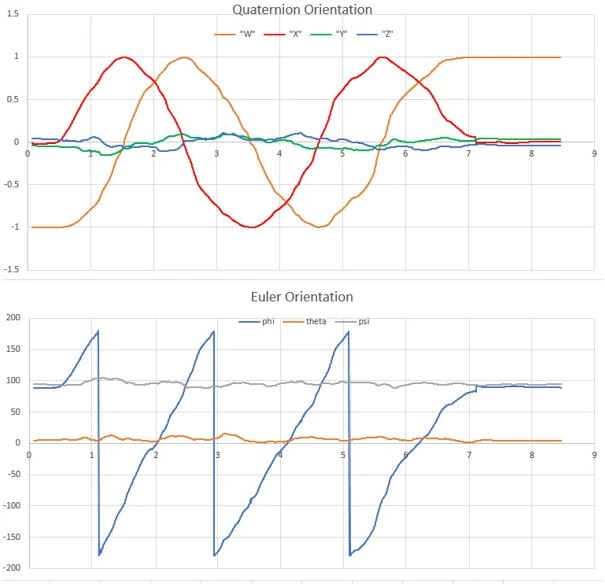
\includegraphics[width=0.5\textwidth]{./Images/euler-quat.JPG}
	\caption{\label{fig:euler-quat}Euler vs Quaternion Orientation \cite{euler-quat}}
\end{figure}

% matthew
\subsubsection{System Data Network}
\noindent The proposed system network for data transmission can be seen pictured below. The ESP32 MCU is the main controller for our system, bringing together the sensor data and the object detection data for the guidance and navigation aspect of FORWARD. The peripheral sensors: IMU, LiDAR, and Sonar are connected to the ESP32 through GPIO and I2C, in which data is transmitted continually. The ESP32 also hosts a wireless network in which the Ameba 82 camera module connects and transmits the object detection data through UDP sockets over WiFi. \\

\noindent The Ameba 82 also plays a crucial role in the networking of our system. It links the object detection data to the ESP32 and the user. As stated above, it transmits the calculated object data to the ESP32, but also transmits the audio of the objects name over Bluetooth to the AfterShokz, which will be to the end user. \\

\begin{figure}[H]
	\centering
	\fbox{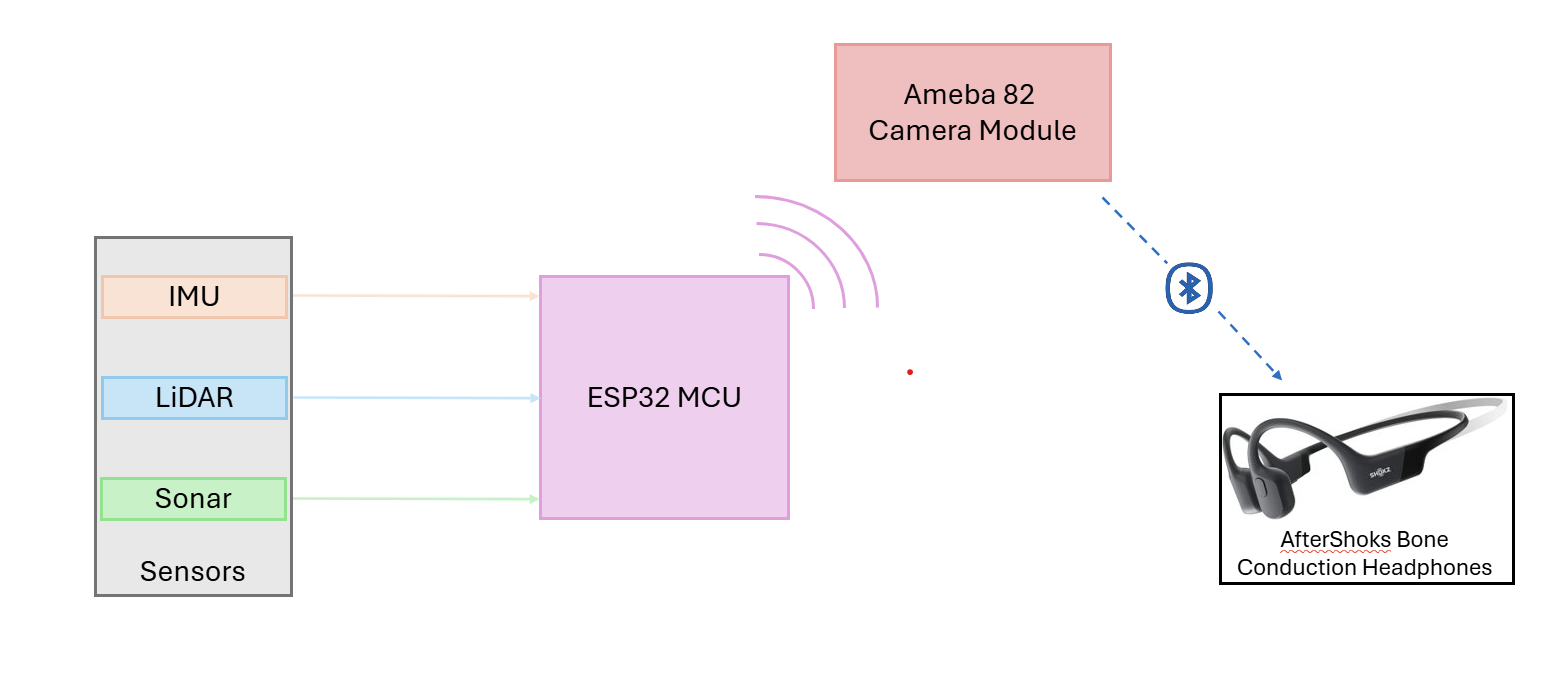
\includegraphics[width=1.0\textwidth]{./Images/System_Network_Arch.png}}
	\caption{\label{fig:System_Network_Arch}System Data Network Architecture}
\end{figure}


% morgan
\subsubsection{Typical steering motor control wiring}

